\upaper{90}{Shamanism --- Medicine Men and Priests}
\uminitoc{The First Shamans --- The Medicine Men}
\uminitoc{Shamanistic Practices}
\uminitoc{The Shamanic Theory of Disease and Death}
\uminitoc{Medicine under the Shamans}
\uminitoc{Priests and Rituals}
\author{Melchizedek}
\vs p090 0:1 The evolution of religious observances progressed from placation, avoidance, exorcism, coercion, conciliation, and propitiation to sacrifice, atonement, and redemption. The technique of religious ritual passed from the forms of the primitive cult through fetishes to magic and miracles; and as ritual became more complex in response to man’s increasingly complex concept of the supermaterial realms, it was inevitably dominated by medicine men, shamans, and priests.
\vs p090 0:2 In the advancing concepts of primitive man the spirit world was eventually regarded as being unresponsive to the ordinary mortal. Only the exceptional among humans could catch the ear of the gods; only the extraordinary man or woman would be heard by the spirits. Religion thus enters upon a new phase, a stage wherein it gradually becomes secondhanded; always does a medicine man, a shaman, or a priest intervene between the religionist and the object of worship. And today most Urantia systems of organized religious belief are passing through this level of evolutionary development.
\vs p090 0:3 Evolutionary religion is born of a simple and all\hyp{}powerful fear, the fear which surges through the human mind when confronted with the unknown, the inexplicable, and the incomprehensible. Religion eventually achieves the profoundly simple realization of an all\hyp{}powerful love, the love which sweeps irresistibly through the human soul when awakened to the conception of the limitless affection of the Universal Father for the sons of the universe. But in between the beginning and the consummation of religious evolution, there intervene the long ages of the shamans, who presume to stand between man and God as intermediaries, interpreters, and intercessors.
\usection{The First Shamans --- The Medicine Men}
\vs p090 1:1 The shaman was the ranking medicine man, the ceremonial fetishman, and the focus personality for all the practices of evolutionary religion. In many groups the shaman outranked the war chief, marking the beginning of the church domination of the state. The shaman sometimes functioned as a priest and even as a priest\hyp{}king. Some of the later tribes had both the earlier shaman\hyp{}medicine men (seers) and the later appearing shaman\hyp{}priests. And in many cases the office of shaman became hereditary.
\vs p090 1:2 Since in olden times anything abnormal was ascribed to spirit possession, any striking mental or physical abnormality constituted qualification for being a medicine man. Many of these men were epileptic, many of the women hysteric, and these two types accounted for a good deal of ancient inspiration as well as spirit and devil possession. Quite a few of these earliest of priests were of a class which has since been denominated paranoiac.
\vs p090 1:3 While they may have practised deception in minor matters, the great majority of the shamans believed in the fact of their spirit possession. Women who were able to throw themselves into a trance or a cataleptic fit became powerful shamanesses; later, such women became prophets and spirit mediums. Their cataleptic trances usually involved alleged communications with the ghosts of the dead. Many female shamans were also professional dancers.
\vs p090 1:4 But not all shamans were self\hyp{}deceived; many were shrewd and able tricksters. As the profession developed, a novice was required to serve an apprenticeship of ten years of hardship and self\hyp{}denial to qualify as a medicine man. The shamans developed a professional mode of dress and affected a mysterious conduct. They frequently employed drugs to induce certain physical states which would impress and mystify the tribesmen. Sleight\hyp{}of\hyp{}hand feats were regarded as supernatural by the common folk, and ventriloquism was first used by shrewd priests. Many of the olden shamans unwittingly stumbled onto hypnotism; others induced autohypnosis by prolonged staring at their navels.
\vs p090 1:5 While many resorted to these tricks and deceptions, their reputation as a class, after all, stood on apparent achievement. When a shaman failed in his undertakings, if he could not advance a plausible alibi, he was either demoted or killed. Thus the honest shamans early perished; only the shrewd actors survived.
\vs p090 1:6 It was shamanism that took the exclusive direction of tribal affairs out of the hands of the old and the strong and lodged it in the hands of the shrewd, the clever, and the farsighted.
\usection{Shamanistic Practices}
\vs p090 2:1 Spirit conjuring was a very precise and highly complicated procedure, comparable to present\hyp{}day church rituals conducted in an ancient tongue. The human race very early sought for superhuman help, for \bibemph{revelation;} and men believed that the shaman actually received such revelations. While the shamans utilized the great power of suggestion in their work, it was almost invariably negative suggestion; only in very recent times has the technique of positive suggestion been employed. In the early development of their profession the shamans began to specialize in such vocations as rain making, disease healing, and crime detecting. To heal diseases was not, however, the chief function of a shamanic medicine man; it was, rather, to know and to control the hazards of living.
\vs p090 2:2 Ancient black art, both religious and secular, was called white art when practised by either priests, seers, shamans, or medicine men. The practitioners of the black art were called sorcerers, magicians, wizards, witches, enchanters, necromancers, conjurers, and soothsayers. As time passed, all such purported contact with the supernatural was classified either as witchcraft or shamancraft.
\vs p090 2:3 Witchcraft embraced the \bibemph{magic} performed by earlier, irregular, and unrecognized spirits; shamancraft had to do with \bibemph{miracles} performed by regular spirits and recognized gods of the tribe. In later times the witch became associated with the devil, and thus was the stage set for the many comparatively recent exhibitions of religious intolerance. Witchcraft was a religion with many primitive tribes.
\vs p090 2:4 The shamans were great believers in the mission of chance as revelatory of the will of the spirits; they frequently cast lots to arrive at decisions. Modern survivals of this proclivity for casting lots are illustrated, not only in the many games of chance, but also in the well\hyp{}known “counting\hyp{}out” rhymes. Once, the person counted out must die; now, he is only \bibemph{it} in some childish game. That which was serious business to primitive man has survived as a diversion of the modern child.
\vs p090 2:5 The medicine men put great trust in signs and omens, such as, “When you hear the sound of a rustling in the tops of the mulberry trees, then shall you bestir yourself.” Very early in the history of the race the shamans turned their attention to the stars. Primitive astrology was a world\hyp{}wide belief and practice; dream interpreting also became widespread. All this was soon followed by the appearance of those temperamental shamanesses who professed to be able to communicate with the spirits of the dead.
\vs p090 2:6 Though of ancient origin, the rain makers, or weather shamans, have persisted right on down through the ages. A severe drought meant death to the early agriculturists; weather control was the object of much ancient magic. Civilized man still makes the weather the common topic of conversation. The olden peoples all believed in the power of the shaman as a rain maker, but it was customary to kill him when he failed, unless he could offer a plausible excuse to account for the failure.
\vs p090 2:7 Again and again did the Caesars banish the astrologers, but they invariably returned because of the popular belief in their powers. They could not be driven out, and even in the XVI century after Christ the directors of Occidental church and state were the patrons of astrology. Thousands of supposedly intelligent people still believe that one may be born under the domination of a lucky or an unlucky star; that the juxtaposition of the heavenly bodies determines the outcome of various terrestrial adventures. Fortunetellers are still patronized by the credulous.
\vs p090 2:8 The Greeks believed in the efficacy of oracular advice, the Chinese used magic as protection against demons, shamanism flourished in India, and it still openly persists in central Asia. It is an only recently abandoned practice throughout much of the world.
\vs p090 2:9 Ever and anon, true prophets and teachers arose to denounce and expose shamanism. Even the vanishing red man had such a prophet within the past 100 years, the Shawnee Tenskwatawa, who predicted the eclipse of the sun in 1806\fnst{The 1955 text reads \bibemph{Teuskwatawa} and \bibemph{1808}.} and denounced the vices of the white man. Many true teachers have appeared among the various tribes and races all through the long ages of evolutionary history. And they will ever continue to appear to challenge the shamans or priests of any age who oppose general education and attempt to thwart scientific progress.\tunemarkup{pictures}{\begin{figure}[H]\centering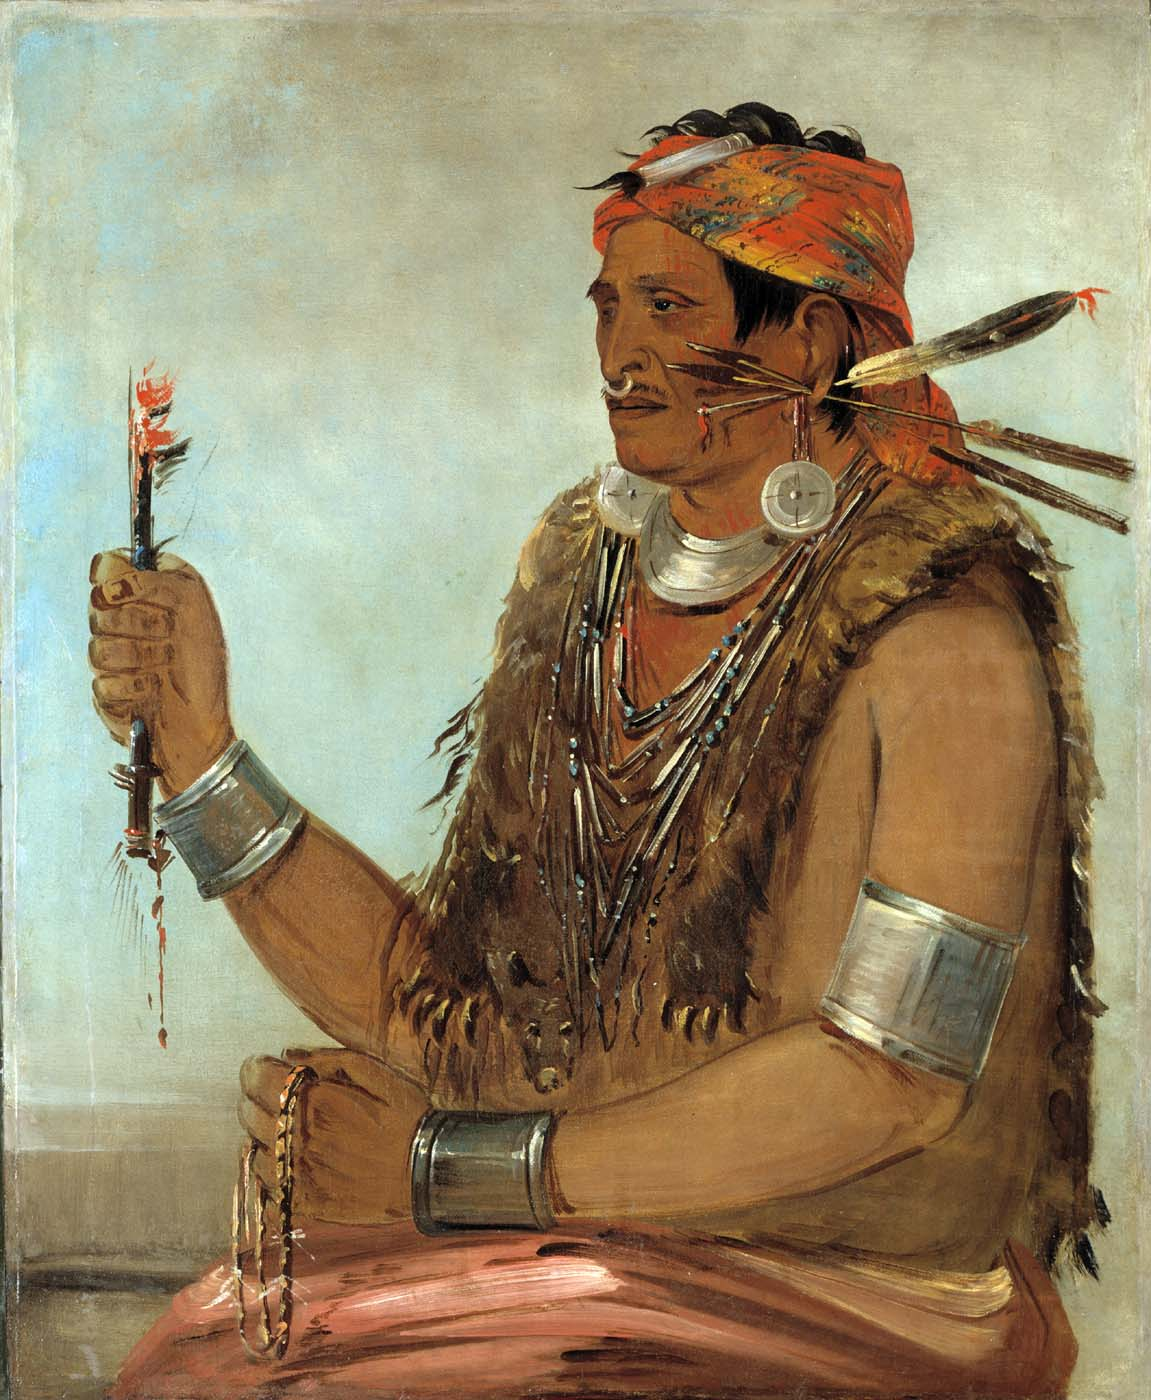
\includegraphics[width=\columnwidth]{images/Tenskwatawa.jpg}\caption{Tenskwatawa, 1830 by George Catlin.}\end{figure}}
\vs p090 2:10 In many ways and by devious methods the olden shamans established their reputations as voices of God and custodians of providence. They sprinkled the newborn with water and conferred names upon them; they circumcised the males. They presided over all burial ceremonies and made due announcement of the safe arrival of the dead in spiritland.
\vs p090 2:11 The shamanic priests and medicine men often became very wealthy through the accretion of their various fees which were ostensibly offerings to the spirits. Not infrequently a shaman would accumulate practically all the material wealth of his tribe. Upon the death of a wealthy man it was customary to divide his property equally with the shaman and some public enterprise or charity. This practice still obtains in some parts of Tibet, where one half the male population belongs to this class of nonproducers.
\vs p090 2:12 The shamans dressed well and usually had a number of wives; they were the original aristocracy, being exempt from all tribal restrictions. They were very often of low\hyp{}grade mind and morals. They suppressed their rivals by denominating them witches or sorcerers and very frequently rose to such positions of influence and power that they were able to dominate the chiefs or kings.
\vs p090 2:13 Primitive man regarded the shaman as a necessary evil; he feared him but did not love him. Early man respected knowledge; he honoured and rewarded wisdom. The shaman was mostly fraud, but the veneration for shamanism well illustrates the premium put upon wisdom in the evolution of the race.
\usection{The Shamanic Theory of Disease and Death}
\vs p090 3:1 Since ancient man regarded himself and his material environment as being directly responsive to the whims of the ghosts and the fancies of the spirits, it is not strange that his religion should have been so exclusively concerned with material affairs. Modern man attacks his material problems directly; he recognizes that matter is responsive to the intelligent manipulation of mind. Primitive man likewise desired to modify and even to control the life and energies of the physical domains; and since his limited comprehension of the cosmos led him to the belief that ghosts, spirits, and gods were personally and immediately concerned with the detailed control of life and matter, he logically directed his efforts to winning the favour and support of these superhuman agencies.
\vs p090 3:2 Viewed in this light, much of the inexplicable and irrational in the ancient cults is understandable. The ceremonies of the cult were primitive man’s attempt to control the material world in which he found himself. And many of his efforts were directed to the end of prolonging life and ensuring health. Since all diseases and death itself were originally regarded as spirit phenomena, it was inevitable that the shamans, while functioning as medicine men and priests, should also have laboured as doctors and surgeons.
\vs p090 3:3 The primitive mind may be handicapped by lack of facts, but it is for all that logical. When thoughtful men observe disease and death, they set about to determine the causes of these visitations, and in accordance with their understanding, the shamans and the scientists have propounded the following theories of affliction:
\vs p090 3:4 \ublistelem{1.}\bibnobreakspace \bibemph{Ghosts --- direct spirit influences.} The earliest hypothesis advanced in explanation of disease and death was that spirits caused disease by enticing the soul out of the body; if it failed to return, death ensued. The ancients so feared the malevolent action of disease\hyp{}producing ghosts that ailing individuals would often be deserted without even food or water. Regardless of the erroneous basis for these beliefs, they did effectively isolate afflicted individuals and prevent the spread of contagious disease.
\vs p090 3:5 \ublistelem{2.}\bibnobreakspace \bibemph{Violence --- obvious causes.} The causes for some accidents and deaths were so easy to identify that they were early removed from the category of ghost action. Fatalities and wounds attendant upon war, animal combat, and other readily identifiable agencies were considered as natural occurrences. But it was long believed that the spirits were still responsible for delayed healing or for the infection of wounds of even “natural” causation. If no observable natural agent could be discovered, the spirit ghosts were still held responsible for disease and death.
\vs p090 3:6 Today, in Africa and elsewhere may be found primitive peoples who kill someone every time a nonviolent death occurs. Their medicine men indicate the guilty parties. If a mother dies in childbirth, the child is immediately strangled --- a life for a life.
\vs p090 3:7 \ublistelem{3.}\bibnobreakspace \bibemph{Magic --- the influence of enemies.} Much sickness was thought to be caused by bewitchment, the action of the evil eye and the magic pointing bow. At one time it was really dangerous to point a finger at anyone; it is still regarded as ill\hyp{}mannered to point. In cases of obscure disease and death the ancients would hold a formal inquest, dissect the body, and settle upon some finding as the cause of death; otherwise the death would be laid to witchcraft, thus necessitating the execution of the witch responsible therefor. These ancient coroner’s inquests saved many a supposed witch’s life. Among some it was believed that a tribesman could die as a result of his own witchcraft, in which event no one was accused.
\vs p090 3:8 \ublistelem{4.}\bibnobreakspace \bibemph{Sin --- punishment for taboo violation.} In comparatively recent times it has been believed that sickness is a punishment for sin, personal or racial. Among peoples traversing this level of evolution the prevailing theory is that one cannot be afflicted unless one has violated a taboo. To regard sickness and suffering as “arrows of the Almighty within them” is typical of such beliefs. The Chinese and Mesopotamians long regarded disease as the result of the action of evil demons, although the Chaldeans also looked upon the stars as the cause of suffering. This theory of disease as a consequence of divine wrath is still prevalent among many reputedly civilized groups of Urantians.
\vs p090 3:9 \ublistelem{5.}\bibnobreakspace \bibemph{Natural causation.} Mankind has been very slow to learn the material secrets of the interrelationship of cause and effect in the physical domains of energy, matter, and life. The ancient Greeks, having preserved the traditions of Adamson’s teachings, were among the first to recognize that all disease is the result of natural causes. Slowly and certainly the unfolding of a scientific era is destroying man’s age\hyp{}old theories of sickness and death. Fever was one of the first human ailments to be removed from the category of supernatural disorders, and progressively the era of science has broken the fetters of ignorance which so long imprisoned the human mind. An understanding of old age and contagion is gradually obliterating man’s fear of ghosts, spirits, and gods as the personal perpetrators of human misery and mortal suffering.
\vs p090 3:10 \pc Evolution unerringly achieves its end: It imbues man with that superstitious fear of the unknown and dread of the unseen which is the scaffolding for the God concept. And having witnessed the birth of an advanced comprehension of Deity, through the co\hyp{}ordinate action of revelation, this same technique of evolution then unerringly sets in motion those forces of thought which will inexorably obliterate the scaffolding, which has served its purpose.
\usection{Medicine under the Shamans}
\vs p090 4:1 The entire life of ancient men was prophylactic; their religion was in no small measure a technique for disease prevention. And regardless of the error in their theories, they were wholehearted in putting them into effect; they had unbounded faith in their methods of treatment, and that, in itself, is a powerful remedy.
\vs p090 4:2 \pc The faith required to get well under the foolish ministrations of one of these ancient shamans was, after all, not materially different from that which is required to experience healing at the hands of some of his later\hyp{}day successors who engage in the nonscientific treatment of disease.
\vs p090 4:3 \pc The more primitive tribes greatly feared the sick, and for long ages they were carefully avoided, shamefully neglected. It was a great advance in humanitarianism when the evolution of shamancraft produced priests and medicine men who consented to treat disease. Then it became customary for the entire clan to crowd into the sickroom to assist the shaman in howling the disease ghosts away. It was not uncommon for a woman to be the diagnosing shaman, while a man would administer treatment. The usual method of diagnosing disease was to examine the entrails of an animal.
\vs p090 4:4 Disease was treated by chanting, howling, laying on of hands, breathing on the patient, and many other techniques. In later times the resort to temple sleep, during which healing supposedly took place, became widespread. The medicine men eventually essayed actual surgery in connection with temple slumber; among the first operations was that of trephining the skull to allow a headache spirit to escape. The shamans learned to treat fractures and dislocations, to open boils and abscesses; the shamanesses became adept at midwifery.
\vs p090 4:5 It was a common method of treatment to rub something magical on an infected or blemished spot on the body, throw the charm away, and supposedly experience a cure. If anyone should chance to pick up the discarded charm, it was believed he would immediately acquire the infection or blemish. It was a long time before herbs and other real medicines were introduced. Massage was developed in connection with incantation, rubbing the spirit out of the body, and was preceded by efforts to rub medicine in, even as moderns attempt to rub liniments in. Cupping and sucking the affected parts, together with bloodletting, were thought to be of value in getting rid of a disease\hyp{}producing spirit.
\vs p090 4:6 Since water was a potent fetish, it was utilized in the treatment of many ailments. For long it was believed that the spirit causing the sickness could be eliminated by sweating. Vapour baths were highly regarded; natural hot springs soon blossomed as primitive health resorts. Early man discovered that heat would relieve pain; he used sunlight, fresh animal organs, hot clay, and hot stones, and many of these methods are still employed. Rhythm was practised in an effort to influence the spirits; the tom\hyp{}toms were universal.
\vs p090 4:7 Among some people disease was thought to be caused by a wicked conspiracy between spirits and animals. This gave rise to the belief that there existed a beneficent plant remedy for every animal\hyp{}caused disease. The red men were especially devoted to the plant theory of universal remedies; they always put a drop of blood in the root hole left when the plant was pulled up.
\vs p090 4:8 Fasting, dieting, and counterirritants were often used as remedial measures. Human secretions, being definitely magical, were highly regarded; blood and urine were thus among the earliest medicines and were soon augmented by roots and various salts. The shamans believed that disease spirits could be driven out of the body by foul\hyp{}smelling and bad\hyp{}tasting medicines. Purging very early became a routine treatment, and the values of raw cocoa and quinine were among the earliest pharmaceutical discoveries.
\vs p090 4:9 The Greeks were the first to evolve truly rational methods of treating the sick. Both the Greeks and the Egyptians received their medical knowledge from the Euphrates valley. Oil and wine was a very early medicine for treating wounds; castor oil and opium were used by the Sumerians. Many of these ancient and effective secret remedies lost their power when they became known; secrecy has always been essential to the successful practice of fraud and superstition. Only facts and truth court the full light of comprehension and rejoice in the illumination and enlightenment of scientific research.
\usection{Priests and Rituals}
\vs p090 5:1 The essence of the ritual is the perfection of its performance; among savages it must be practised with exact precision. It is only when the ritual has been correctly carried out that the ceremony possesses compelling power over the spirits. If the ritual is faulty, it only arouses the anger and resentment of the gods. Therefore, since man’s slowly evolving mind conceived that the \bibemph{technique of ritual} was the decisive factor in its efficacy, it was inevitable that the early shamans should sooner or later evolve into a priesthood trained to direct the meticulous practice of the ritual. And so for tens of thousands of years endless rituals have hampered society and cursed civilization, have been an intolerable burden to every act of life, every racial undertaking.
\vs p090 5:2 Ritual is the technique of sanctifying custom; ritual creates and perpetuates myths as well as contributing to the preservation of social and religious customs. Again, ritual itself has been fathered by myths. Rituals are often at first social, later becoming economic and finally acquiring the sanctity and dignity of religious ceremonial. Ritual may be personal or group in practice --- or both --- as illustrated by prayer, dancing, and drama.
\vs p090 5:3 Words become a part of ritual, such as the use of terms like amen and selah. The habit of swearing, profanity, represents a prostitution of former ritualistic repetition of holy names. The making of pilgrimages to sacred shrines is a very ancient ritual. The ritual next grew into elaborate ceremonies of purification, cleansing, and sanctification. The initiation ceremonies of the primitive tribal secret societies were in reality a crude religious rite. The worship technique of the olden mystery cults was just one long performance of accumulated religious ritual. Ritual finally developed into the modern types of social ceremonials and religious worship, services embracing prayer, song, responsive reading, and other individual and group spiritual devotions.
\vs p090 5:4 \pc The priests evolved from shamans up through oracles, diviners, singers, dancers, weathermakers, guardians of religious relics, temple custodians, and foretellers of events, to the status of actual directors of religious worship. Eventually the office became hereditary; a continuous priestly caste arose.
\vs p090 5:5 As religion evolved, priests began to specialize according to their innate talents or special predilections. Some became singers, others prayers, and still others sacrificers; later came the orators --- preachers. And when religion became institutionalized, these priests claimed to “hold the keys of heaven.”
\vs p090 5:6 The priests have always sought to impress and awe the common people by conducting the religious ritual in an ancient tongue and by sundry magical passes so to mystify the worshippers as to enhance their own piety and authority. The great danger in all this is that the ritual tends to become a substitute for religion.
\vs p090 5:7 The priesthoods have done much to delay scientific development and to hinder spiritual progress, but they have contributed to the stabilization of civilization and to the enhancement of certain kinds of culture. But many modern priests have ceased to function as directors of the ritual of the worship of God, having turned their attention to theology --- the attempt to define God.
\vs p090 5:8 It is not denied that the priests have been a millstone about the neck of the races, but the true religious leaders have been invaluable in pointing the way to higher and better realities.
\vsetoff
\vs p090 5:9 [Presented by a Melchizedek of Nebadon.]
\quizlink
